\subsection{High throughput binding affinity calculator}

(Stefan/Jumana)

HT-BAC is a workflow system that uses RADICAL-Cybertools to implement ESMACS protocol, consisting of concurrent multi-stage consecutive MD runs followed by post processing steps. HT-BAC uses the EnTK API to express this workflow, which provides the required high-throughput capabilities. 

\begin{figure}[tb]
\centering
  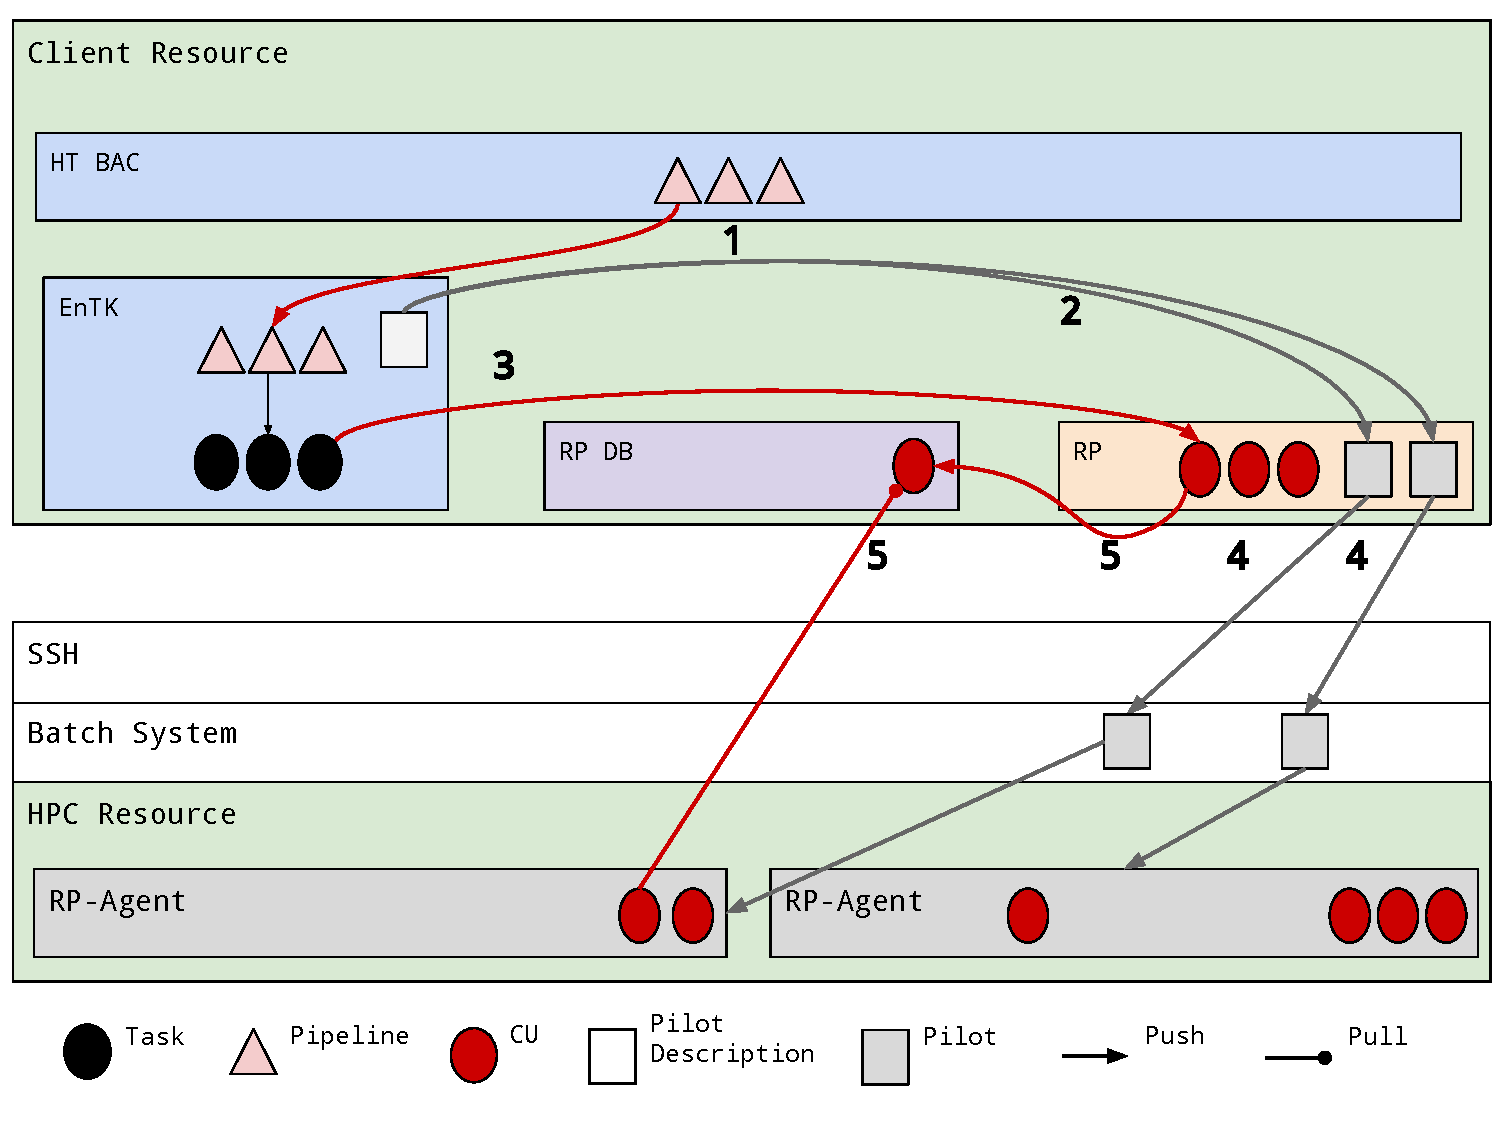
\includegraphics[width=0.6\textwidth]{FIGURES/ht-bac-rp_integration.pdf}
  \caption{\bf Integration between HT-BAC workflow system and EnTK. Numbers indicate the temporal sequence of execution. RADICAL-Pilot (RP) database (DB) can be deployed on any host reachable from the resources.}
   \label{figure:ht-bac_rp}
\end{figure}
